% Shared section: used by paper-ieee.tex, paper-lncs.tex and report.tex.
% Use \sect / \subsect for headings (see README), never \section directly.

\sect{System Design}\label{system-design}

\subsect{Sensing and computation placement}\label{sensing-and-computation-placement}

The prototype combines Sony WH-1000XM5 consumer headphones, a Samsung Galaxy Watch and a Tauri desktop application \cite{tauri}. The headphones provide head orientation through the open-source sony-head-tracker interface \cite{sonyheadtracker}. The watch streams raw green, red and infrared PPG through the Samsung Health Sensor SDK \cite{samsungsdk}, along with three-axis acceleration and angular velocity. Both devices act only as sensors; training, inference and every interaction decision happen on the laptop. A camera is used while recording to produce reference labels from MediaPipe hand landmarks \cite{mediapipe}, but it plays no part in normal use.

\iffull
The watch can connect over Bluetooth Low Energy or Wi-Fi. Samples keep the timestamps assigned on the watch rather than the time they arrive at the laptop. We treat transport, buffering and resampling as separate steps: the model works on a 50\,Hz grid, but that does not mean every sensor was sampled at 50\,Hz or that the detector makes a decision every 20\,ms. We record the actual input and decision rates for each experiment.
\else
The watch connects over Bluetooth Low Energy or Wi-Fi, and samples keep their watch timestamps. The model works on a 50\,Hz grid, which does not imply that every sensor was sampled at that rate.
\fi

\begin{widefigure}
\centering
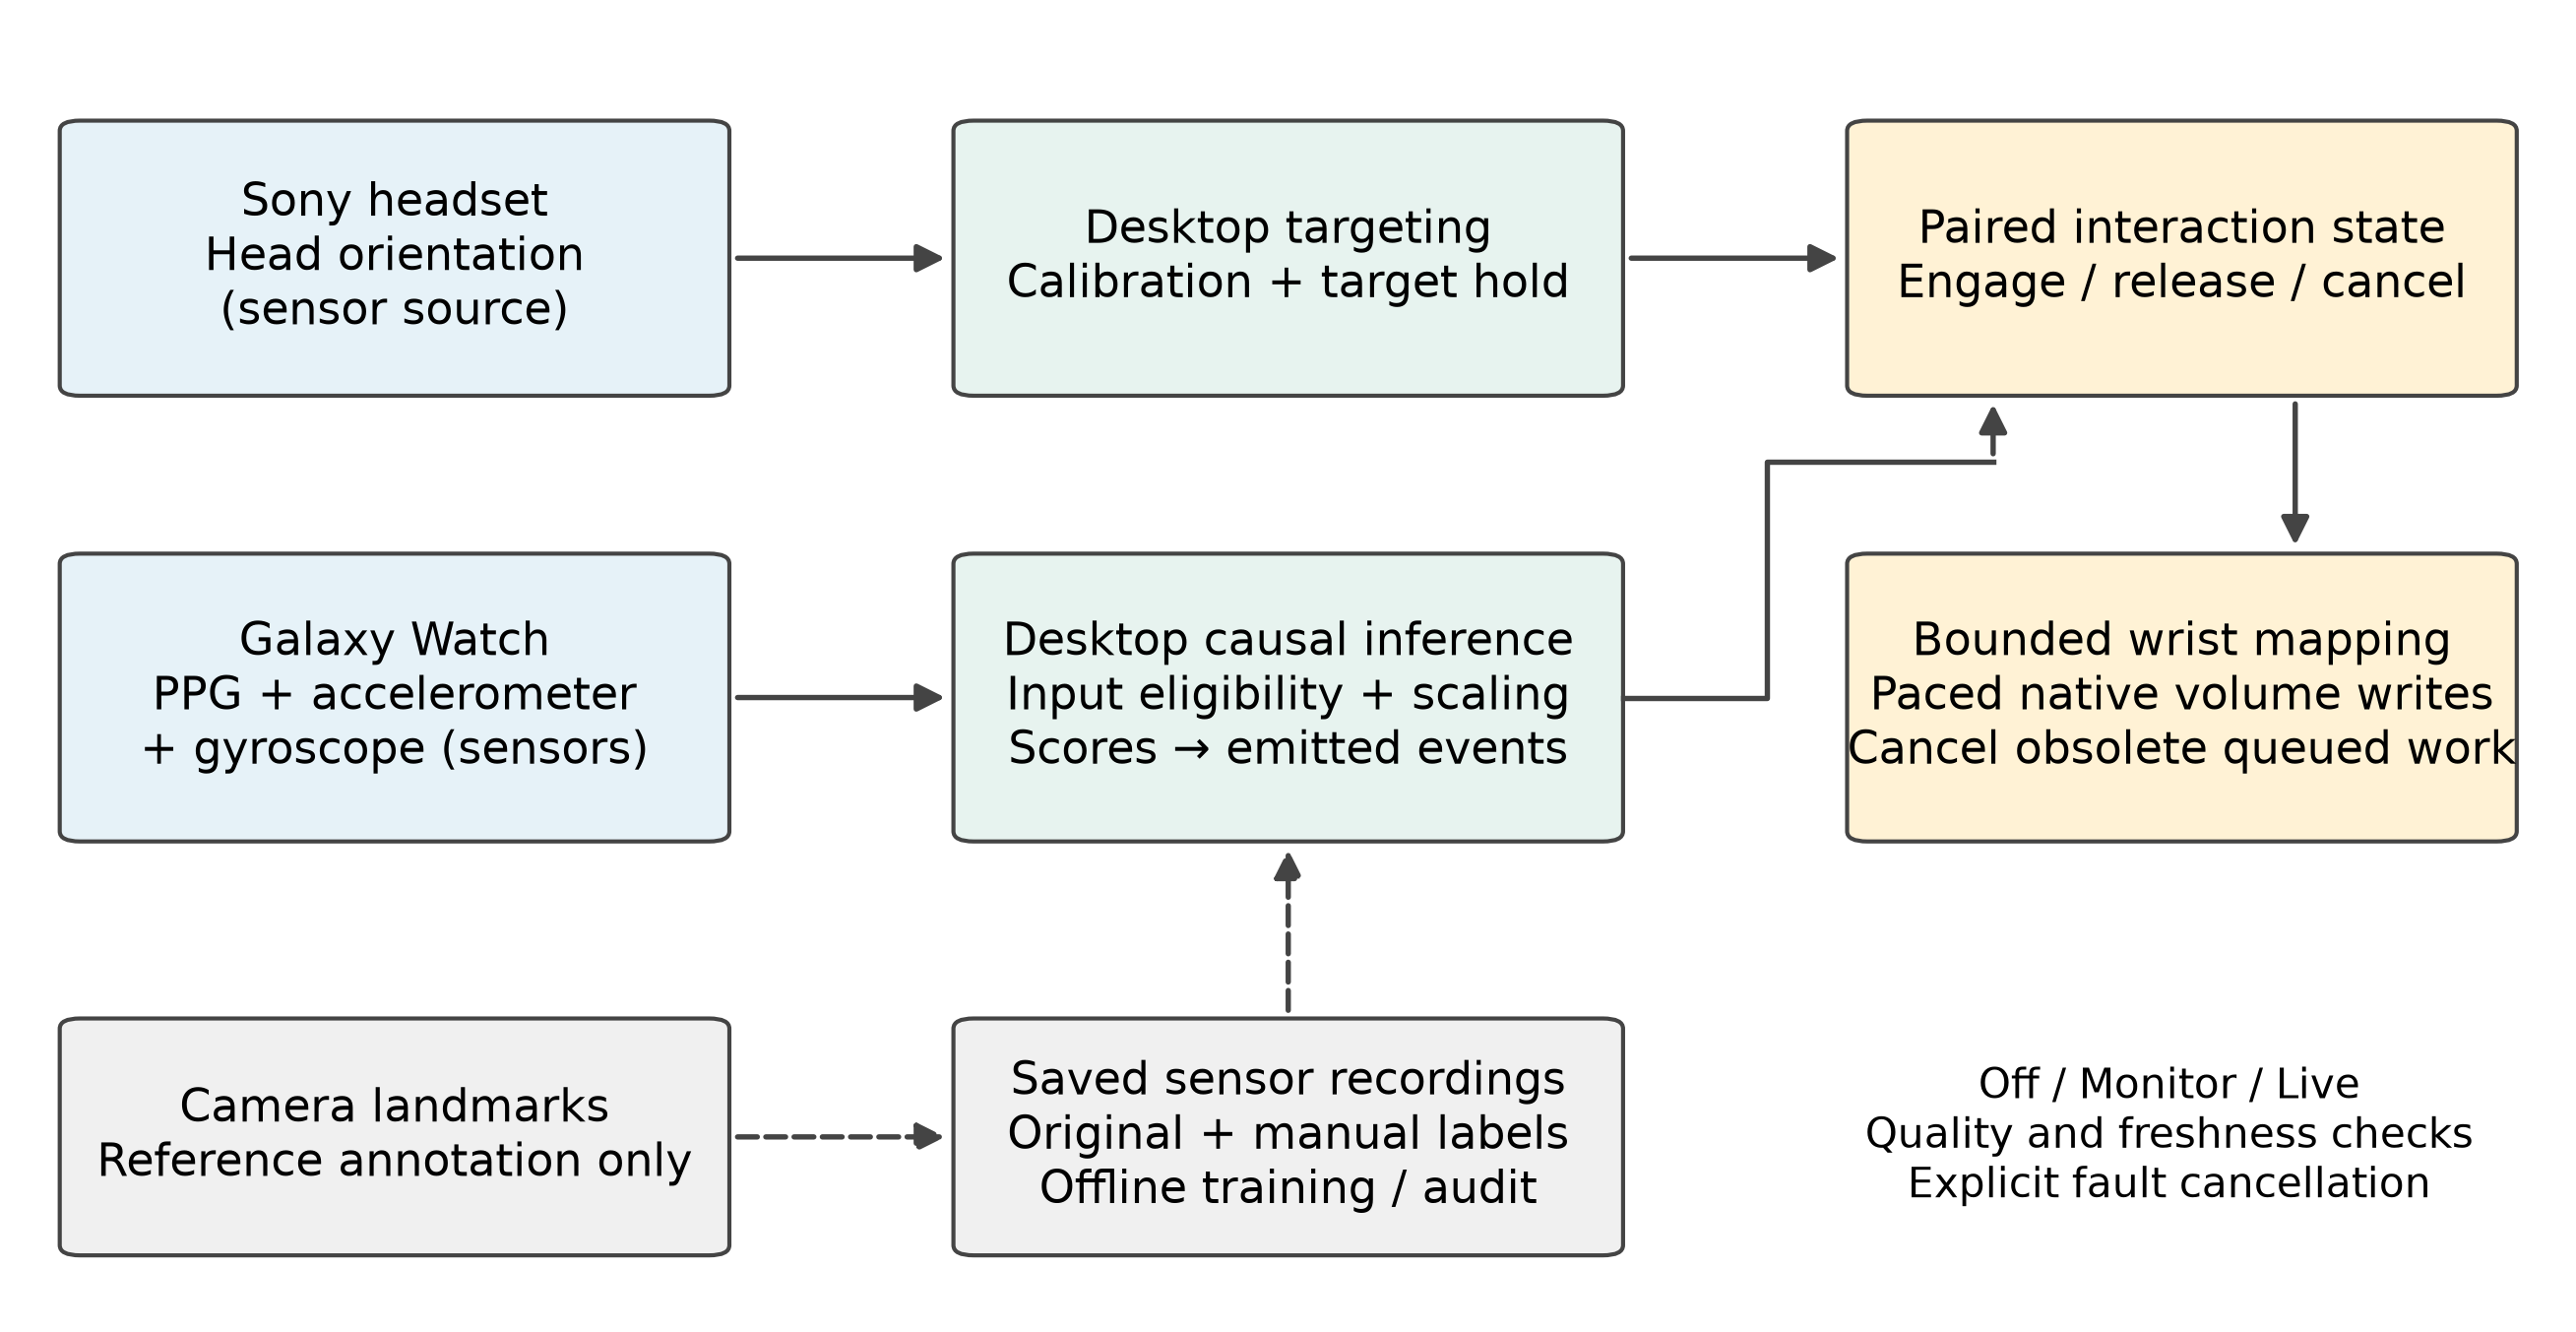
\includegraphics[width=1\linewidth,height=\textheight,keepaspectratio,alt={System architecture: headphone orientation supplies target selection, watch PPG and IMU supply desktop causal inference, and a paired interaction policy controls bounded volume writes; camera reference annotation is an offline path.}]{figures/system-overview.png}
\caption[System overview]{System overview. Head orientation selects the target, watch PPG and IMU feed a causal detector on the laptop, and a paired grab/release policy drives bounded volume changes. The camera is used only to create reference labels.}\label{fig-system}
\end{widefigure}

\subsect{Head targeting and paired interaction}\label{head-targeting-and-paired-interaction}

Head orientation is mapped to a calibrated point on the screen. This is head-directed selection; we do not track the eyes. While the head rests on the volume target, a fresh pinch-in event starts a grab. Wrist roll relative to the grab position then sets an absolute volume level, and a separate pinch-out event ends the grab. Silence from the detector is never taken to mean the fingers have opened, and further pinch-in events during a grab are ignored.

\iffull
The reason for this split is that a pinch is a momentary event, while adjusting the volume takes time. Letting one classifier score drive the output directly would tie the two together. Instead, recognition, interaction state and cancellation are handled separately. A grab also ends when the head leaves the target, when the user presses Escape, when the data become stale or are rejected, when the mode changes or when the model is replaced. If a start and a release arrive together, the release wins.
\else
Because a pinch is momentary while adjusting the volume takes time, recognition, interaction state and cancellation are handled separately. A grab also ends when the head leaves the target, on Escape, on stale or rejected data, on a mode change or on model replacement, and a simultaneous release beats a start.
\fi

\subsect{Bounded actuation and failure handling}\label{bounded-actuation-and-failure-handling}

\iffull
The application has three modes: Off, Monitor and Live. Monitor shows what the system would do without touching the system volume, and a saved Live setting is lowered to Monitor at startup, so the system never acts on its own after a restart. All output goes through the interaction policy; the web view cannot inject gesture events directly. Each model is checked against its declared hash and input format before loading. A matching hash shows the file is intact, not that the model works well.
\else
Off, Monitor and Live modes control actuation: Monitor shows what the system would do without changing the volume, and a saved Live setting starts as Monitor. All output passes through the interaction policy, and each model is checked against its declared hash and input format before loading. The wrist mapper bounds the rate and range of change, and queued volume writes are tagged with their grab so stale writes are discarded; a write already sent to the operating system still completes.
\fi

\iffull
The wrist mapper records a reference angle when the grab starts, limits how fast the level can change and clamps it to the valid range. Every queued volume write is tagged with the grab it belongs to, so writes left over from an earlier grab are discarded. A write that has already reached the operating system will still complete, so cancellation stops further changes rather than undoing the last one. Long-run transport reliability, battery use and cancellation timing on real hardware still need to be measured.

\fi